\documentclass[12pt, a4paper, oneside]{article}\usepackage[]{graphicx}\usepackage[]{color}
%% maxwidth is the original width if it is less than linewidth
%% otherwise use linewidth (to make sure the graphics do not exceed the margin)
\makeatletter
\def\maxwidth{ %
  \ifdim\Gin@nat@width>\linewidth
    \linewidth
  \else
    \Gin@nat@width
  \fi
}
\makeatother

\definecolor{fgcolor}{rgb}{0.345, 0.345, 0.345}
\newcommand{\hlnum}[1]{\textcolor[rgb]{0.686,0.059,0.569}{#1}}%
\newcommand{\hlstr}[1]{\textcolor[rgb]{0.192,0.494,0.8}{#1}}%
\newcommand{\hlcom}[1]{\textcolor[rgb]{0.678,0.584,0.686}{\textit{#1}}}%
\newcommand{\hlopt}[1]{\textcolor[rgb]{0,0,0}{#1}}%
\newcommand{\hlstd}[1]{\textcolor[rgb]{0.345,0.345,0.345}{#1}}%
\newcommand{\hlkwa}[1]{\textcolor[rgb]{0.161,0.373,0.58}{\textbf{#1}}}%
\newcommand{\hlkwb}[1]{\textcolor[rgb]{0.69,0.353,0.396}{#1}}%
\newcommand{\hlkwc}[1]{\textcolor[rgb]{0.333,0.667,0.333}{#1}}%
\newcommand{\hlkwd}[1]{\textcolor[rgb]{0.737,0.353,0.396}{\textbf{#1}}}%

\usepackage{framed}
\makeatletter
\newenvironment{kframe}{%
 \def\at@end@of@kframe{}%
 \ifinner\ifhmode%
  \def\at@end@of@kframe{\end{minipage}}%
  \begin{minipage}{\columnwidth}%
 \fi\fi%
 \def\FrameCommand##1{\hskip\@totalleftmargin \hskip-\fboxsep
 \colorbox{shadecolor}{##1}\hskip-\fboxsep
     % There is no \\@totalrightmargin, so:
     \hskip-\linewidth \hskip-\@totalleftmargin \hskip\columnwidth}%
 \MakeFramed {\advance\hsize-\width
   \@totalleftmargin\z@ \linewidth\hsize
   \@setminipage}}%
 {\par\unskip\endMakeFramed%
 \at@end@of@kframe}
\makeatother

\definecolor{shadecolor}{rgb}{.97, .97, .97}
\definecolor{messagecolor}{rgb}{0, 0, 0}
\definecolor{warningcolor}{rgb}{1, 0, 1}
\definecolor{errorcolor}{rgb}{1, 0, 0}
\newenvironment{knitrout}{}{} % an empty environment to be redefined in TeX

\usepackage{alltt} % Paper size, default font size and one-sided paper
%\graphicspath{{./Figures/}} % Specifies the directory where pictures are stored
%\usepackage[dcucite]{harvard}
\usepackage{amsmath}
\usepackage{setspace}
\usepackage{pdflscape}
\usepackage{rotating}
\usepackage[flushleft]{threeparttable}
\usepackage{multirow}
\usepackage[comma, sort&compress]{natbib}% Use the natbib reference package - read up on this to edit the reference style; if you want text (e.g. Smith et al., 2012) for the in-text references (instead of numbers), remove 'numbers' 
\usepackage{graphicx}
%\bibliographystyle{plainnat}
\bibliographystyle{agsm}
\usepackage[colorlinks = true, citecolor = blue, linkcolor = blue]{hyperref}
%\hypersetup{urlcolor=blue, colorlinks=true} % Colors hyperlinks in blue - change to black if annoying
%\renewcommand[\harvardurl]{URL: \url}
\usepackage{listings}
\usepackage{color}
\definecolor{mygrey}{gray}{0.95}
\lstset{backgroundcolor=\color{mygrey}}
\IfFileExists{upquote.sty}{\usepackage{upquote}}{}
\begin{document}
\title{Machine Learning}
\author{Rob Hayward}
\date{\today}
\maketitle
\subsection*{Introduction}
These are the notes from  \href{https://class.coursera.org/ml-006}{the Peng Machine Learning course}. 

Introduction to the methods and model representations.  This is an example of \emph{supervised learning}.  There is a training set that is used to develop a model.  \lstinline{m} is the number  of training examples, \lstinline{x} are the input variables or features, \lstinline{y} are the output variables \lstinline{(x, y)} is a training example, $(x^{(i)}), 
y^{(i)}$ is a training set.

The aim is to get the parameters of a hypothesis.  The hypothesis is 
\begin{equation}
h_{\theta}(x) = \theta_0 + \theta_1 x
\end{equation}

This is a linear regression model. The aim is to chose the values of the parameters $\theta_0$ and $\theta_1$ to minimise the difference between actual and forecast values. 

Objective function
\begin{equation}
\text{minimise}_{\theta_0, \theta_1)} \text{   for} \frac{1}{2m} \sum (h_0(x) - y)^2
\end{equation}

The cost function
\begin{equation}
J(\theta_0, \theta_1) = \frac{1}{2m} \sum_{i = 1}^m (h_0 x^{(i)} - y^{(i)})^2
\end{equation}

This is also called the \emph{squared error function}

A simplified version can just look at one of the parameters $(\theta_1)$.  This would be a line through the origin. There are two functions:  $h_{\theta}(x)$ is a function of $x$; $J(\theta_1)$ is a function of $\theta_1$.  

\begin{knitrout}
\definecolor{shadecolor}{rgb}{0.969, 0.969, 0.969}\color{fgcolor}
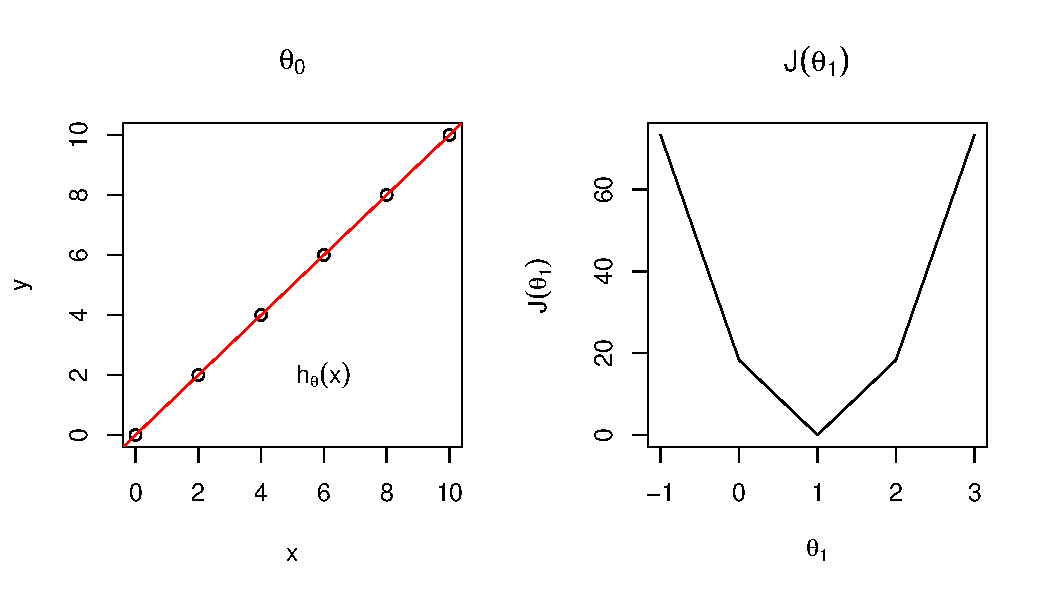
\includegraphics[width=\maxwidth]{figure/cost} 

\end{knitrout}

Clearly the value of $\theta_1$ that will minimise the cost function is one.  

Now we have the same case with both papameters changing. This can be shown using \emph{contour plots} or \emph{contour figures}. 


\href{http://econometricsense.blogspot.co.uk/2011/11/regression-via-gradient-descent-in-r.html}{Econometric Sense}
\begin{knitrout}
\definecolor{shadecolor}{rgb}{0.969, 0.969, 0.969}\color{fgcolor}\begin{kframe}
\begin{alltt}
\hlstd{x0} \hlkwb{<-} \hlkwd{c}\hlstd{(}\hlnum{1}\hlstd{,} \hlnum{1}\hlstd{,} \hlnum{1}\hlstd{,} \hlnum{1}\hlstd{,} \hlnum{1}\hlstd{)}  \hlcom{# column of 1's}
\hlstd{x1} \hlkwb{<-} \hlkwd{c}\hlstd{(}\hlnum{1}\hlstd{,} \hlnum{2}\hlstd{,} \hlnum{3}\hlstd{,} \hlnum{4}\hlstd{,} \hlnum{5}\hlstd{)}  \hlcom{# original x-values}
\hlcom{# create the x- matrix of explanatory variables}
\hlstd{x} \hlkwb{<-} \hlkwd{as.matrix}\hlstd{(}\hlkwd{cbind}\hlstd{(x0, x1))}
\hlcom{# create the y-matrix of dependent variables}
\hlstd{y} \hlkwb{<-} \hlkwd{as.matrix}\hlstd{(}\hlkwd{c}\hlstd{(}\hlnum{3}\hlstd{,} \hlnum{7}\hlstd{,} \hlnum{5}\hlstd{,} \hlnum{11}\hlstd{,} \hlnum{14}\hlstd{))}
\hlstd{m} \hlkwb{<-} \hlkwd{nrow}\hlstd{(y)}
\hlcom{# implement feature scaling}
\hlstd{x.scaled} \hlkwb{<-} \hlstd{x}
\hlstd{x.scaled[,} \hlnum{2}\hlstd{]} \hlkwb{<-} \hlstd{(x[,} \hlnum{2}\hlstd{]} \hlopt{-} \hlkwd{mean}\hlstd{(x[,} \hlnum{2}\hlstd{]))}\hlopt{/}\hlkwd{sd}\hlstd{(x[,} \hlnum{2}\hlstd{])}
\hlcom{# analytical results with matrix algebra}
\hlkwd{solve}\hlstd{(}\hlkwd{t}\hlstd{(x)} \hlopt \hlstd{x)} \hlopt \hlkwd{t}\hlstd{(x)} \hlopt \hlstd{y}  \hlcom{# w/o feature scaling}
\end{alltt}
\begin{verbatim}
##    [,1]
## x0  0.2
## x1  2.6
\end{verbatim}
\begin{alltt}
\hlkwd{solve}\hlstd{(}\hlkwd{t}\hlstd{(x.scaled)} \hlopt \hlstd{x.scaled)} \hlopt \hlkwd{t}\hlstd{(x.scaled)} \hlopt \hlstd{y}  \hlcom{# w/ feature scaling}
\end{alltt}
\begin{verbatim}
##     [,1]
## x0 8.000
## x1 4.111
\end{verbatim}
\begin{alltt}
\hlcom{# results using canned lm function match results above}
\hlkwd{summary}\hlstd{(}\hlkwd{lm}\hlstd{(y} \hlopt{~} \hlstd{x[,} \hlnum{2}\hlstd{]))}  \hlcom{# w/o feature scaling}
\end{alltt}
\begin{verbatim}
## 
## Call:
## lm(formula = y ~ x[, 2])
## 
## Residuals:
##    1    2    3    4    5 
##  0.2  1.6 -3.0  0.4  0.8 
## 
## Coefficients:
##             Estimate Std. Error t value Pr(>|t|)  
## (Intercept)    0.200      2.132    0.09    0.931  
## x[, 2]         2.600      0.643    4.04    0.027 *
## ---
## Signif. codes:  0 '***' 0.001 '**' 0.01 '*' 0.05 '.' 0.1 ' ' 1
## 
## Residual standard error: 2.03 on 3 degrees of freedom
## Multiple R-squared:  0.845,	Adjusted R-squared:  0.793 
## F-statistic: 16.4 on 1 and 3 DF,  p-value: 0.0272
\end{verbatim}
\begin{alltt}
\hlkwd{summary}\hlstd{(}\hlkwd{lm}\hlstd{(y} \hlopt{~} \hlstd{x.scaled[,} \hlnum{2}\hlstd{]))}  \hlcom{# w/feature scaling}
\end{alltt}
\begin{verbatim}
## 
## Call:
## lm(formula = y ~ x.scaled[, 2])
## 
## Residuals:
##    1    2    3    4    5 
##  0.2  1.6 -3.0  0.4  0.8 
## 
## Coefficients:
##               Estimate Std. Error t value Pr(>|t|)   
## (Intercept)      8.000      0.909    8.80   0.0031 **
## x.scaled[, 2]    4.111      1.017    4.04   0.0272 * 
## ---
## Signif. codes:  0 '***' 0.001 '**' 0.01 '*' 0.05 '.' 0.1 ' ' 1
## 
## Residual standard error: 2.03 on 3 degrees of freedom
## Multiple R-squared:  0.845,	Adjusted R-squared:  0.793 
## F-statistic: 16.4 on 1 and 3 DF,  p-value: 0.0272
\end{verbatim}
\begin{alltt}
\hlcom{# define the gradient function dJ/dtheata: 1/m * (h(x)-y))*x where h(x) =}
\hlcom{# x*theta in matrix form this is as follows:}
\hlstd{grad} \hlkwb{<-} \hlkwa{function}\hlstd{(}\hlkwc{x}\hlstd{,} \hlkwc{y}\hlstd{,} \hlkwc{theta}\hlstd{) \{}
    \hlstd{gradient} \hlkwb{<-} \hlstd{(}\hlnum{1}\hlopt{/}\hlstd{m)} \hlopt{*} \hlstd{(}\hlkwd{t}\hlstd{(x)} \hlopt \hlstd{((x} \hlopt \hlkwd{t}\hlstd{(theta))} \hlopt{-} \hlstd{y))}
    \hlkwd{return}\hlstd{(}\hlkwd{t}\hlstd{(gradient))}
\hlstd{\}}
\hlcom{# define gradient descent update algorithm}
\hlstd{grad.descent} \hlkwb{<-} \hlkwa{function}\hlstd{(}\hlkwc{x}\hlstd{,} \hlkwc{maxit}\hlstd{) \{}
    \hlstd{theta} \hlkwb{<-} \hlkwd{matrix}\hlstd{(}\hlkwd{c}\hlstd{(}\hlnum{0}\hlstd{,} \hlnum{0}\hlstd{),} \hlkwc{nrow} \hlstd{=} \hlnum{1}\hlstd{)}  \hlcom{# Initialize the parameters}
    \hlstd{alpha} \hlkwb{=} \hlnum{0.05}  \hlcom{# set learning rate}
    \hlkwa{for} \hlstd{(i} \hlkwa{in} \hlnum{1}\hlopt{:}\hlstd{maxit) \{}
        \hlstd{theta} \hlkwb{<-} \hlstd{theta} \hlopt{-} \hlstd{alpha} \hlopt{*} \hlkwd{grad}\hlstd{(x, y, theta)}
    \hlstd{\}}
    \hlkwd{return}\hlstd{(theta)}
\hlstd{\}}
\hlcom{# results without feature scaling}
\hlkwd{print}\hlstd{(}\hlkwd{grad.descent}\hlstd{(x,} \hlnum{1000}\hlstd{))}
\end{alltt}
\begin{verbatim}
##          x0  x1
## [1,] 0.2001 2.6
\end{verbatim}
\begin{alltt}
\hlcom{# results with feature scaling}
\hlkwd{print}\hlstd{(}\hlkwd{grad.descent}\hlstd{(x.scaled,} \hlnum{1000}\hlstd{))}
\end{alltt}
\begin{verbatim}
##      x0    x1
## [1,]  8 4.111
\end{verbatim}
\begin{alltt}
\hlcom{# -----------------------------------------------------------------------}
\hlcom{# cost and convergence intuition}
\hlcom{# -----------------------------------------------------------------------}
\hlcom{# typically we would iterate the algorithm above until the change in the}
\hlcom{# cost function (as a result of the updated b0 and b1 values) was extremely}
\hlcom{# small value 'c'. C would be referred to as the set 'convergence' criteria.}
\hlcom{# If C is not met after a given # of iterations, you can increase the}
\hlcom{# iterations or change the learning rate 'alpha' to speed up convergence}
\hlcom{# get results from gradient descent}
\hlstd{beta} \hlkwb{<-} \hlkwd{grad.descent}\hlstd{(x,} \hlnum{1000}\hlstd{)}
\hlcom{# define the 'hypothesis function'}
\hlstd{h} \hlkwb{<-} \hlkwa{function}\hlstd{(}\hlkwc{xi}\hlstd{,} \hlkwc{b0}\hlstd{,} \hlkwc{b1}\hlstd{) \{}
    \hlstd{b0} \hlopt{+} \hlstd{b1} \hlopt{*} \hlstd{xi}
\hlstd{\}}
\hlcom{# define the cost function}
\hlstd{cost} \hlkwb{<-} \hlkwd{t}\hlstd{(}\hlkwd{mat.or.vec}\hlstd{(}\hlnum{1}\hlstd{, m))}
\hlkwa{for} \hlstd{(i} \hlkwa{in} \hlnum{1}\hlopt{:}\hlstd{m) \{}
    \hlstd{cost[i,} \hlnum{1}\hlstd{]} \hlkwb{<-} \hlstd{(}\hlnum{1}\hlopt{/}\hlstd{(}\hlnum{2} \hlopt{*} \hlstd{m))} \hlopt{*} \hlstd{(}\hlkwd{h}\hlstd{(x[i,} \hlnum{2}\hlstd{], beta[}\hlnum{1}\hlstd{,} \hlnum{1}\hlstd{], beta[}\hlnum{1}\hlstd{,} \hlnum{2}\hlstd{])} \hlopt{-} \hlstd{y[i, ])}\hlopt{^}\hlnum{2}
\hlstd{\}}
\hlstd{totalCost} \hlkwb{<-} \hlkwd{colSums}\hlstd{(cost)}
\hlkwd{print}\hlstd{(totalCost)}
\end{alltt}
\begin{verbatim}
## [1] 1.24
\end{verbatim}
\begin{alltt}
\hlcom{# save this as Cost1000}
\hlstd{cost1000} \hlkwb{<-} \hlstd{totalCost}
\hlcom{# change iterations to 1001 and compute cost1001}
\hlstd{beta} \hlkwb{<-} \hlstd{(}\hlkwd{grad.descent}\hlstd{(x,} \hlnum{1001}\hlstd{))}
\hlstd{cost} \hlkwb{<-} \hlkwd{t}\hlstd{(}\hlkwd{mat.or.vec}\hlstd{(}\hlnum{1}\hlstd{, m))}
\hlkwa{for} \hlstd{(i} \hlkwa{in} \hlnum{1}\hlopt{:}\hlstd{m) \{}
    \hlstd{cost[i,} \hlnum{1}\hlstd{]} \hlkwb{<-} \hlstd{(}\hlnum{1}\hlopt{/}\hlstd{(}\hlnum{2} \hlopt{*} \hlstd{m))} \hlopt{*} \hlstd{(}\hlkwd{h}\hlstd{(x[i,} \hlnum{2}\hlstd{], beta[}\hlnum{1}\hlstd{,} \hlnum{1}\hlstd{], beta[}\hlnum{1}\hlstd{,} \hlnum{2}\hlstd{])} \hlopt{-} \hlstd{y[i, ])}\hlopt{^}\hlnum{2}
\hlstd{\}}
\hlstd{cost1001} \hlkwb{<-} \hlkwd{colSums}\hlstd{(cost)}
\hlcom{# does this difference meet your convergence criteria?}
\hlkwd{print}\hlstd{(cost1000} \hlopt{-} \hlstd{cost1001)}
\end{alltt}
\begin{verbatim}
## [1] 1.515e-11
\end{verbatim}
\end{kframe}
\end{knitrout}




\end{document}
